\documentclass[a4paper,12pt]{article}
\usepackage{graphicx}
\usepackage{amsmath, amssymb, amsthm}
\usepackage{xcolor}
\definecolor{mydarkblue}{RGB}{0, 0, 139}
\usepackage[colorlinks=true, linkcolor=mydarkblue, citecolor=mydarkblue, urlcolor=mydarkblue]{hyperref}
\usepackage[ngerman]{babel}
\usepackage[
  backend=biber,
  citestyle=authoryear,
  bibstyle=numeric,
  natbib=true,
  hyperref=true
]{biblatex}
\usepackage{amsfonts}
\usepackage{booktabs}
\usepackage{verbatim}

\title{{Wynns $\rho$-Algorithmus}}
\author{Lucas Posern}
\date{Juli 2025}
\addbibresource{quellen.bib}
\graphicspath{{figures/}}
\numberwithin{equation}{section}

% Definition von Referenzbefehlen
\newcommand{\secref}[1]{\hyperref[#1]{Abschnitt~\ref*{#1}}}
\newcommand{\figref}[1]{\hyperref[#1]{Abbildung~\ref*{#1}}}
\newcommand{\eqnref}[1]{\hyperref[#1]{Gleichung~\eqref{#1}}}
\newcommand{\lemref}[1]{\hyperref[#1]{Lemma~\ref*{#1}}}
\newcommand{\sref}[1]{\hyperref[#1]{Satz~\ref*{#1}}}

\newtheorem{satz}{Satz}[section]
\newtheorem{lemma}[satz]{Lemma}
\newtheorem{definition}[satz]{Definition}
\theoremstyle{remark}
\newtheorem*{bemerkung}{Bemerkung}

\begin{document}
\maketitle
\thispagestyle{empty}
\newpage
\thispagestyle{empty}
\tableofcontents
\newpage
\pagenumbering{arabic} % Start der arabischen Nummerierung
\setcounter{page}{1}   



\section{Einführung}\label{sec:einleitung}
Allgemeine Aussagen zu Konvergenzproblemen und deren Beschleunigungen entnehmen wir aus [\cite[194-199]{weniger1996nonlinear}].
In vielen Bereichen der numerischen Mathematik und der wissenschaftlichen Berechnung spielen iterative Verfahren eine zentrale Rolle. Sie dienen dazu, Lösungen von Gleichungen, Reihen oder Fixpunktproblemen Schritt für Schritt zu approximieren. Ein häufiges Problem solcher Verfahren ist jedoch die oft langsame Konvergenz, die den Rechenaufwand erheblich erhöht und in der Praxis die Effizienz und Anwendbarkeit einschränkt. Hier setzt die Konvergenzbeschleunigung an. Sie umfasst Methoden, die darauf abzielen, die Geschwindigkeit der Annäherung an den Grenzwert deutlich zu verbessern.

Wynns $\rho$-Algorithmus, benannt nach Peter Wynn, der ihn in den 1950er Jahren entwickelte, ist eine dieser Methoden zur Konvergenzbeschleunigung. Der Algorithmus entstand ursprünglich aus der Herausforderung heraus, um die Handhabung langsam konvergierender oder gar divergierender Reihen und Folgen zu verbessern. In der Praxis zeigte sich, dass viele klassische Reihenentwicklungen und iterative Verfahren oft erst nach einer sehr großen Anzahl von Schritten brauchbare Ergebnisse liefern, sofern sie überhaupt in endlicher Zeit konvergieren. Der $\rho$-Algorithmus bietet hier eine elegante Möglichkeit, durch rekursive Transformationen die Konvergenzrate signifikant zu erhöhen.

Der Wynnsche $\rho$-Algorithmus ist hierbei eine Erweiterung des Wynnschen $\epsilon$-Algorithmus. Sie unterscheiden sich zwar nur geringfügig, sind aber dadurch für verschiedene Konvergenzklassen anwendbar.

Im weiteren Verlauf dieser Arbeit wird der Wynnsche $\rho$-Algorithmus detailliert vorgestellt, seine mathematischen Grundlagen erläutert sowie typische Anwendungsbeispiele gezeigt, die seine Bedeutung und Leistungsfähigkeit im Bereich der Konvergenzbeschleunigung verdeutlichen.

\section{Notwendigkeit des $\rho$-Algorithmus}\label{sec:notwendigkeit}
Für Aussagen zum Wynn-$\epsilon$-Algorithmus beziehen wir uns auf [\cite{wynn1966convergence}].\\

Der $\epsilon$-Algorithmus, eingeführt von Peter Wynn (1956), machte einen wesentlichen Fortschritt für die Konvergenzbeschleunigung durch seine elegante Rekursion:
\[
\epsilon_{k+1}^{(n)} = \epsilon_{k-1}^{(n+1)} + \frac{1}{\epsilon_k^{(n+1)} - \epsilon_k^{(n)}}
\]
Dennoch kam das Verfahren an Grenzen:
\begin{enumerate}
\item \textbf{Nicht immer erfolgreich}: Für logarithmische Konvergenz  versagt der $\epsilon$-Algorithmus.
\item \textbf{Parameterstarre}: Die feste Koeffizientenstruktur ($+1$ im Zähler) lässt keine Anpassung an unterschiedliche asymptotische Entwicklungen zu.
\end{enumerate}
Der $\rho$-Algorithmus (Wynn, 1966) behebt diese Defizite durch eine fundamentale strukturelle Modifikation:
\[
\rho_{k+1}^{(n)} = \rho_{k-1}^{(n+1)} + \frac{k+1}{\rho_k^{(n+1)} - \rho_k^{(n)}}
\]
Seine Innovationskraft liegt in folgenden Kernaspekten:
\begin{enumerate}
\item \textbf{Beschleunigung für andere Folgen}: Dem $\rho$-Algorithmus gelingt die Konvergenzbeschleunigung für logarithmisch konvergente Folgen durch die dynamische Skalierung des Zählers mit $k+1$.
\item \textbf{Parametrisierbarkeit}: Die Erweiterung zum $\rho(\gamma,p)$-Algorithmus (\secref{subsubsec:mod1}) ermöglicht die Anpassung an beliebige Entwicklungen der Form $s_n \sim s + n^\theta(c_0 + c_1/n + \cdots)$.
\end{enumerate}

\section{Wynns $\rho$-Algorithmus}\label{sec:wynn}
\subsection{Idee}\label{subsec:idee}

Der Wynnsche $\rho$-Algorithmus ist eine Technik zur Beschleunigung der Konvergenz von Zahlenfolgen. Insbesondere bei langsam konvergenten Folgen oder bei Reihen, deren Summen schwierig direkt zu berechnen sind, bietet der Algorithmus eine effektive Möglichkeit zur Verbesserung der numerischen Genauigkeit. Er gehört zu den sogenannten nichtlinearen Transformationen und ist insbesondere für logarithmisch konvergente Folgen geeignet.

Der Grundgedanke hinter Konvergenzbeschleunigungsverfahren ist, aus einer gegebenen Folge $\{s_n\}$ eine neue Folge $\{\rho_n\}$ zu erzeugen, die gegen denselben Grenzwert konvergiert, jedoch deutlich schneller.

\subsection{Definition}\label{subsec:def}
Wir nutzen die Definition des $\rho$-Algorithmus aus [\cite[34-35]{weniger1996nonlinear}].\\
Der $\rho$-Algorithmus basiert auf einer rekursiven Konstruktion einer Tabelle ähnlich dem $\varepsilon$-Algorithmus. Gegeben sei eine Folge $\{s_n\}_{n=0}^{\infty}$, so wird die Rho-Tabelle $\rho^{(k)}_n$ wie folgt rekursiv definiert:

\begin{align}
\rho^{(n)}_{-1} &= 0 \quad\\
\rho^{(n)}_0 &= s_n \\
\rho^{(n)}_{k+1} &= \rho^{(n+1)}_{k} + \frac{x_{n+k+1}-x_{n}}{\rho^{(n+1)}_{k} - \rho^{(n)}_k}, \quad k \ge 0 \label{eq:rhodef}
\end{align}
Voraussetzung für die Berechnung ist, dass die Interpolationspunkte $x_n$ eine aufsteigende divergente Folge bilden:
\begin{gather*}
x_0<x_1<\cdots\\
\lim_{n\rightarrow\infty}x_{n}=\infty
\end{gather*}
Im Fall, dass die Interpolationspunkte einfach der Nummer des Folgenglieds entsprechen ($x_n = n$) lässt sich der Algorithmus auch so definieren:
\begin{align}
\rho^{(-1)}_n &= 0 \quad\\
\rho^{(0)}_n &= s_n \\
\rho^{(k+1)}_n &= \rho^{(k-1)}_{n+1} + \frac{k+1}{\rho^{(k)}_{n+1} - \rho^{(k)}_n}, \quad k \ge 0 \label{eq:rho_rek}
\end{align}
Der Wert $\rho^{(2k)}_0$ ergibt die transformierte Näherung an den Grenzwert. Die ungeraden Indizes $\rho^{(2k+1)}_n$ besitzen dabei nur indirekt eine Bedeutung für die Approximation.

\subsection{Beispiel}\label{subsec:beispiel}
Als einfaches Beispiel betrachten wir die einfache Folge
\begin{gather*}
s_n=\frac{2+3x_n}{1+x_n}, \quad x_n=n+1 \\
s=\lim_{n\rightarrow\infty}{s_n}=\lim_{n\rightarrow\infty}{\frac{2+3(n+1)}{1+(n+1)}}=3    
\end{gather*}
Die Folgenglieder lauten:
\begin{align*}
    s_0&=\frac{2+3x_n}{1+x_n}=\frac{2+3(0+1)}{1+(0+1)}=\frac{5}{2}=2.5\\
    s_1&=[...]=\frac{8}{3}\approx2.667\\
    s_2&= [...]=2.75\\
    s_3&= [...]=2.8
\end{align*}
$\rho$-Iterationen:
\begin{align*}
    \rho_{-1}^{(n)}&=0\\
    \rho_{0}^{(n)}&=s_n\\
    \rho_{k+1}^{(n)}&=\rho_{k-1}^{(n+1)}+\frac{x_{n+k+1}-x_{n}}{\rho_{k}^{(n+1)}-\rho_{k}^{(n)}}
\end{align*}
Fülle die $\rho$-Tabelle:
\begin{table}[h!]
\centering
\begin{tabular}{c@{\hspace{1.5cm}}c@{\hspace{1.5cm}}c}
$n$ & $\rho_{-1}^{(n)}$ & $\rho_{0}^{(n)}$ \\
\midrule
    0 & 0 & 2,500 \\
    1 & 0 & 2,667 \\
    2 & 0 & 2,750 \\
    3 & 0 & 2,800 \\
\end{tabular}
\end{table}
\\\\
Stufe 1, k=0: $\rho_{1}^{(n)}=\rho_{-1}^{(n+1)}+\frac{x_{n+1}-x_{n}}{\rho_{0}^{(n+1)}-\rho_{0}^{(n)}}$
\begin{align*}
    \rho_{1}^{(0)}&=0+\frac{x_{1}-x_{0}}{s_1-s_{0}}=\frac{2-1}{2,667-2,500}=\frac{1}{0,1667}\approx6\\
    \rho_{1}^{(1)}&=0+\frac{x_{2}-x_{1}}{s_2-s_{1}}=\frac{3-2}{2,750-2,667}=\frac{1}{0,0833}\approx12\\
    \rho_{1}^{(2)}&=0+\frac{x_{3}-x_{2}}{s_3-s_{2}}=\frac{4-3}{2,800-2,750}=\frac{1}{0,05}=20
\end{align*}
Stufe 2, k=1: $\rho_{2}^{(n)}=\rho_{0}^{(n+1)}+\frac{x_{n+1+1}-x_{n}}{\rho_{1}^{(n+1)}-\rho_{1}^{(n)}}$
\begin{align*}
    \rho_{2}^{(0)}&=s_1+\frac{x_{2}-x_{0}}{\rho_1^{(1)}-\rho_1^{(0)}}=2,667+\frac{3-1}{12-6}=2,667+\frac{2}{6}\approx3\\
    \rho_{2}^{(1)}&=s_2+\frac{x_{3}-x_{1}}{\rho_1^{(2)}-\rho_1^{(1)}}=2,750+\frac{4-2}{20-12}=2,750+\frac{2}{8}=3
\end{align*}
$\rho$-Tabelle jetzt:
\begin{table}[h!]
\centering
\begin{tabular}{c@{\hspace{1.1cm}}c@{\hspace{1.1cm}}c@{\hspace{1.1cm}}c@{\hspace{1.1cm}}c}
$n$ & $\rho_{-1}^{(n)}$ & $\rho_{0}^{(n)}$ & $\rho_{1}^{(n)}$ & $\rho_{2}^{(n)}$\\
\midrule
    0 & 0 & 2,500 & 6 & 3\\
    1 & 0 & 2,667 & 12 & 3\\
    2 & 0 & 2,750 & 12\\
    3 & 0 & 2,800 \\
\end{tabular}
\end{table}
\\
$\implies$ Die Beschleunigung war erfolgreich.\\\\
Die transformierten Werte $\rho_{2}^{(0)}$ und $\rho_{2}^{(1)}$ entsprechen dem Grenzwert $s=3$. Das ist eine starke Verbesserung in der Beschleunigung der Konvergenz.

\subsection{Beschleunigung}\label{subsec:beweis}
Den Beweis zur Beschleunigung einer Folge durch den $\rho$-Algorithmus nehmen wir aus [\cite[522-525]{osada1996acceleration}].\\
In dieser Arbeit beweisen wir, dass der $\rho$-Algorithmus die Konvergenz einer Folge
\[
s_n \sim s + n^{\theta}(c_0  + \frac{c_1}{n} + \frac{c_2}{n^2} + \dots) \quad \text{für } n \to \infty
\]
genau dann beschleunigt, wenn $\theta$ eine negative ganze Zahl ist. Außerdem zeigen wir, dass der $\rho$-Algorithmus keine lineare Konvergenz beschleunigen kann.

\begin{definition}[Assoziierte Folge]\label{subsec:assoz}
\textnormal{Um das asymptotische Verhalten des $\rho$-Algorithmus zu beschreiben, verwenden wir eine verwandte Folge.} Für gegebenes $\theta \notin \big\{0,1\big\}$ und gegebenes $c \ne 0$ definieren wir eine Folge $(C_k)_{k=-1,0,1,\dots}$ durch:
\begin{align*}
C_{-1} &= 0 \\
C_0 &= c \\
C_{2k-1} &= C_{2k-3} + \frac{2k - 1}{\theta C_{2k-2}}, \quad k = 1, 2, \dots\\
C_{2k} &= C_{2k-2} + \frac{2k}{(1 - \theta) C_{2k-1}}, \quad k = 1, 2, \dots
\end{align*}
Diese Folge $(C_k)$ nennen wir die assoziierte Folge des $\rho$-Algorithmus bezüglich $\theta$ und $c$.
\end{definition}

\begin{lemma}\label{lemma}
Die assoziierte Folge kann explizit dargestellt werden als
\[
C_{2k-1} = 
\begin{cases}
\frac{1}{c\theta}, & k = 1, \\
\frac{k(2-\theta)\cdots(k-\theta)}{c\theta(1+\theta)\cdots(k-1+\theta)}, & k > 1,
\end{cases}
\]
\[
C_{2k} = \frac{c(1+\theta)\cdots(k+\theta)}{(1-\theta)\cdots(k-\theta)},
\]
wobei
\[
k \in 
\begin{cases}
k\in\mathbb{N}, & \theta \notin \mathbb{Z}, \\
k< \theta, & \theta \in \mathbb{N}, \\
k\leq |\theta|, & -\theta \in \mathbb{N}.
\end{cases}
\]
\end{lemma}

\begin{proof}
Der Beweis erfolgt durch Induktion. Die Darstellungen sind wahr für $k = 1$, weil 
\[
C_1 = C_{-1} + \frac{1}{c\theta} = \frac{1}{c\theta}, \quad \text{und} \quad 
C_2 = C_0 + \frac{2}{(1-\theta)C_1} = \frac{c(1+\theta)}{1-\theta}.
\]
Nehmen wir an, dass sie für $k > 1$ wahr sind. Durch die Induktionsannahme erhalten wir
\begin{align*}
C_{2k+1} &= C_{2k-1} + \frac{2k + 1}{\theta C_{2k}} \\
&= \frac{k(2-\theta)\cdots(k-\theta)}{c\theta(1+\theta)\cdots(k+\theta)} 
+ \frac{(2k+1)(1-\theta)\cdots(k-\theta)}{c\theta(1+\theta)\cdots(k-1+\theta)} \\
&= \frac{(k+1)(2-\theta)\cdots(k-\theta)(k+1-\theta)}{c\theta(1+\theta)\cdots(k+\theta)}.
\end{align*}
Ebenso gilt
\[
C_{2k+2} = \frac{c(1+\theta)(2+\theta)\cdots(k+1+\theta)}{(1-\theta)\cdots(k+1-\theta)}.
\]

\end{proof}

\begin{satz}\label{satz1}
Sei \((s_n)\) eine Folge mit
\[
s_n \sim s + n^{\theta} \left( c_0 + \frac{c_1}{n} + \frac{c_2}{n^2} + \cdots \right), \quad n \to \infty
\]
\textit{mit \(\operatorname{Re} \theta < 0\), \(c_0 \neq 0\) und Konstanten \(c_k\). Sei \((C_k)\) die assoziierte Folge zu \(\theta\) und \(c_0\), und}
\[
A = (1 - \theta) \left( -\frac{1}{2} + \frac{c_1}{c_0 \theta} \right).
\]
\textit{Dann gilt für festes \(k \in \mathbb{N}\) mit \(\theta \neq -1, \dots, 1 - k\):}
\begin{align*}
\rho_{2k-1}^{(n)} &= C_{2k-1} (n + k)^{1 - \theta} \left( 1 + \frac{A}{n + k} \right) + O\left( (n + k)^{-1 - \theta} \right), \\
\rho_{2k}^{(n)} &= s + C_{2k} (n + k)^{\theta} \left( 1 + \frac{c_1}{c_0 (n + k)} \right) + O\left( (n + k)^{\theta - 2} \right).
\end{align*}
\end{satz}
\begin{proof}
Wir führen eine vollständige Induktion über \(k\). 

\paragraph{Induktionsanfang (\(k = 1\)):}
Für \(\rho_1^{(n)}\) und \(\rho_2^{(n)}\) verwenden wir die Definition des \(\rho\)-Algorithmus:
\[
\rho_1^{(n)} = n + \frac{1}{s_{n+1} - s_n}, \quad
\rho_2^{(n)} = s_{n+1} + \frac{2}{(s_{n+2} - s_{n+1})^{-1} - (s_{n+1} - s_n)^{-1}}.
\]
Mit der asymptotischen Entwicklung von \(s_n\) und binomischer Entwicklung erhalten wir:
\[
s_{n+1} - s_n = c_0 \theta (n + 1)^{\theta - 1} \left[ 1 - \frac{A}{n + 1} + \kappa_1 (n + 1)^{-2} + O\left( (n + 1)^{\theta - 3} \right) \right],
\]
wobei \(\kappa_1 = -\frac{(1 - \theta)(2 - \theta)}{12} + \frac{c_1 (1 - \theta)}{2c_0} + \frac{c_2}{c_0 \theta}\). Einsetzen in \(\rho_1^{(n)}\) liefert:
\[
\rho_1^{(n)} = \frac{1}{c_0 \theta} (n + 1)^{1 - \theta} \left[ 1 + \frac{A}{n + 1} + \kappa_2 (n + 1)^{-2} + O\left( (n + 1)^{-3} \right) \right] + n,
\]
mit \(\kappa_2 = A^2 - \kappa_1\). Da \(C_1 = \frac{1}{c_0 \theta}\) (aus \lemref{lemma}) und \((n + 1)^{1 - \theta}\) dominiert \(n\) für \(\operatorname{Re} \theta < 0\), folgt:
\[
\rho_1^{(n)} = C_1 (n + 1)^{1 - \theta} \left( 1 + \frac{A}{n + 1} \right) + O\left( (n + 1)^{-1 - \theta} \right).
\]
Analog zeigt man für \(\rho_2^{(n)}\):
\[
\rho_2^{(n)} = s + C_2 (n + 1)^{\theta} \left( 1 + \frac{c_1}{c_0 (n + 1)} \right) + O\left( (n + 1)^{\theta - 2} \right),
\]
wobei \(C_2 = \frac{c_0 (1 + \theta)}{1 - \theta}\) (\lemref{lemma}).

\paragraph{Induktionsschritt (\(k \to k + 1\)):} 
Annahme: Die Aussagen gelten für ein beliebiges \(k \geq 1\).

\begin{enumerate}
\item {Zeige \(\rho_{2k+1}^{(n)}\):} \\
Nach Definition des \(\rho\)-Algorithmus gilt:
\[
\rho_{2k+1}^{(n)} = \rho_{2k-1}^{(n+1)} + \frac{2k + 1}{\rho_{2k}^{(n+1)} - \rho_{2k}^{(n)}}.
\]
Aus der Induktionsannahme für \(\rho_{2k}^{(m)}\) folgt:
\[
\rho_{2k}^{(n+1)} - \rho_{2k}^{(n)} = \theta C_{2k} (n + k + 1)^{\theta - 1} \left[ 1 - \frac{A}{n + k + 1} \right] + O\left( (n + k + 1)^{\theta - 3} \right).
\]
Für \(\rho_{2k-1}^{(n+1)}\) gilt:
\[
\rho_{2k-1}^{(n+1)} = C_{2k-1} (n + k + 1)^{1 - \theta} \left( 1 + \frac{A}{n + k + 1} \right) + O\left( (n + k + 1)^{-1 - \theta} \right).
\]
Einsetzen und Umformen ergibt:
\[
\rho_{2k+1}^{(n)} = \underbrace{C_{2k-1} + \frac{2k + 1}{\theta C_{2k}}}_{= C_{2k+1} \text{ (Rekursion aus \lemref{lemma})}} (n + k + 1)^{1 - \theta} \left( 1 + \frac{A}{n + k + 1} \right) + R_n,
\]
wobei der Restterm \(R_n = O\left( (n + k + 1)^{-1 - \theta} \right)\) alle Fehler absorbiert. Somit:
\[
\rho_{2k+1}^{(n)} = C_{2k+1} (n + k + 1)^{1 - \theta} \left( 1 + \frac{A}{n + k + 1} \right) + O\left( (n + k + 1)^{-1 - \theta} \right).
\]

\item {Zeige \(\rho_{2k+2}^{(n)}\):} \\
Analog gilt:
\[
\rho_{2k+2}^{(n)} = \rho_{2k}^{(n+1)} + \frac{2k + 2}{\rho_{2k+1}^{(n+1)} - \rho_{2k+1}^{(n)}}.
\]
Aus dem soeben Gezeigten folgt:
\[
\rho_{2k+1}^{(n+1)} - \rho_{2k+1}^{(n)} = (1 - \theta) C_{2k+1} (n + k + 1)^{-\theta} \left[ 1 - \frac{c_1}{c_0 (n + k + 1)} \right] + O\left( (n + k + 1)^{-2 - \theta} \right).
\]
Mit Induktionsannahme für \(\rho_{2k}^{(n+1)}\) folgt:
\[
\rho_{2k}^{(n+1)} = s + C_{2k} (n + k + 1)^{\theta} \left( 1 + \frac{c_1}{c_0 (n + k + 1)} \right) + O\left( (n + k + 1)^{\theta - 2} \right).
\]
Einsetzen und Ausnutzen der Rekursion \(C_{2k+2} = C_{2k} + \frac{2k + 2}{(1 - \theta) C_{2k+1}}\) (\lemref{lemma}) liefert:
\[
\rho_{2k+2}^{(n)} = s + C_{2k+2} (n + k + 1)^{\theta} \left( 1 + \frac{c_1}{c_0 (n + k + 1)} \right) + O\left( (n + k + 1)^{\theta - 2} \right). \qedhere
\]
\end{enumerate}

\end{proof}





\begin{satz}[Beschleunigung]\label{satz2}
\textit{Sei $(s_n)$ eine Folge mit
\[
s_n \sim s + n^{\theta}(c_0 + \frac{c_1}{n} + \frac{c_2}{n^2} + \cdots), \quad \text{für } n \to \infty
\]
mit $c_0 \ne 0$.
Der $\rho$-Algorithmus beschleunigt die Konvergenz der Folge $(s_n)$ genau dann, wenn $\theta$ eine negative ganze Zahl ist.}
\end{satz}

\begin{proof}
Nach \sref{satz1} gilt für jedes feste $k$:
\begin{align*}
\lim_{n \to \infty} \frac{\rho_{2k}^{(n)} - s}{s_{n+2k} - s} &= \lim_{n \to \infty}\frac{s+C_{2k}(n+k)^{\theta}(1+\frac{c_0}{c_1(n+k)})+O((n+k)^{\theta-2})-s}{s+(n+2k)^\theta(c_0+\frac{c_1}{n+2k}+\frac{c_2}{(n+2k)^2}+\dots)-s}\\
&=\lim_{n \to \infty}\frac{C_{2k}(n+k)^{\theta}(1+\frac{c_0}{c_1(n+k)})+O((n+k)^{\theta-2})}{(n+2k)^\theta c_0(1+\frac{c_1}{c_0(n+2k)}+\frac{c_2}{c_0(n+2k)^2}+\dots)}\\
&=\frac{C_{2k}}{c_0} 
\end{align*}
Im Normalfall ist $\frac{C_{2k}}{c_0}\neq0$ und der Algorithmus konvergiert nicht schneller als die Originalfolge. Nach \lemref{lemma} wissen wir aber:

\begin{center}
$\theta = -k$ für $k \in \mathbb{N}$ $\implies$ $C_0\ne0,\dots,C_{2k-2}\ne0$ und $C_{2k} = 0$
\end{center}
Daraus folgt also direkt, dass $\lim_{n \to \infty} \frac{\rho_{2k}^{(n)} - s}{s_{n+2k} - s}=\frac{C_{2k}}{c_0}=0$. Damit beschleunigt der $\rho$-Algorithmus die Folge $s_n$.

\end{proof}




\subsection{Schwächen}\label{subsec:schwächen}
Für die folgenden beiden Sätze beziehen wir uns auf [\cite[526-527]{osada1996acceleration}]. Sie werden grundlegend nur auf die Definition \eqref{eq:rho_rek} angewandt (Zähler $= k+1$).
\begin{satz}\label{satz3}
\textnormal{Wir verwenden hier eine alternative Definition für lineare Konvergenz.}
\textit{Sei $(s_n)$ eine gegen $s$ konvergente Folge mit $e_n = s_n - s$, wobei gilt:
\[
e_{n+1} = (\lambda + \varepsilon_n)e_n, \quad \lambda\in[-1,1)\setminus\{0\}, \space \varepsilon_n \to 0.
\]
Dann gilt:
\[
\rho^{(n)}_{2k} = s + (-1)^k e_{n+k} + O(e_{n+k} \varepsilon_{n,k-1}),
\]
mit $\varepsilon_{n,k} = \max\{ |\varepsilon_n|, \ldots, |\varepsilon_{n+k}| \}$.}
\end{satz}
\begin{proof}
Der Beweis dazu findet sich in [\cite[526-527]{osada1996acceleration}]. Die Idee des Beweises ist, zunächst eine rekursive, alternierende Folge $D_k$ zu definieren und anschließend mittels Induktion zu zeigen, dass der $\rho$-Algorithmus in Abhängigkeit von dieser Folge dargestellt werden kann.
\end{proof}

\begin{satz}\label{satz4}
\textit{Der $\rho$-Algorithmus kann lineare Konvergenz nicht beschleunigen.}
\end{satz}

\begin{proof}
Nach \sref{satz3} ergibt sich:
\begin{align*}
    \lim_{n \to \infty} \frac{ \rho^{(n)}_{2k} - s }{ s_{n+2k} - s } &= \lim_{n \to \infty} \frac{ s + (-1)^k e_{n+k} + O(e_{n+k} \varepsilon_{n,k-1}) - s }{ s + e_{n+2k} - s } \\
&=\lim_{n \to \infty} \frac{(-1)^k e_{n+k} + O(e_{n+k} \varepsilon_{n,k-1})}{e_{n+2k}} \\
&=\frac{(-1)^k\lambda^k e_{n}}{\lambda^{2k}e_{n}} \\
&=\frac{(-1)^k}{\lambda^k} \ne 0.
\end{align*}
Damit wird keine Beschleunigung erzielt.

\end{proof}
\newpage
% \subsection{Implementierung in Python}\label{subsec:implementierung}
% Der folgende Code stellt eine Implementierung in Python da. Es wird sehr einfach die $\rho$-Tabelle aufgebaut, dazu werden Details für Rundungsfehler berücksichtigt.
% \begin{verbatim}
% def wynn_rho(s, max_k):
%     n = len(s)
%     rho_table = [[None] * (max_k + 1) for _ in range(n)]

%     # Initialisiere die 0-te Spalte (Ordnung 0)
%     for i in range(n):
%         rho_table[i][0] = s[i]

%     # Fülle die Tabelle für k von 1 bis max_k
%     for k in range(1, max_k + 1):
%         for i in range(n - k):
%             # Berechne den Nenner
%             nenner = rho_table[i + 1][k - 1] - rho_table[i][k - 1]

%             # Vermeide Division durch Null
%             if abs(denom) < 1e-12:
%                 rho_table[i][k] = 0.0
%             else:
%                 if k == 1:
%                     # Sonderfall für k=1: rho_{-1} = 0
%                     rho_table[i][k] = 1 / nenner
%                 else:
%                     # Allgemeine Rekursion
%                     rho_table[i][k] = rho_table[i + 1][k - 2] + (k) / nenner

%     return rho_table
% \end{verbatim}
\newpage
\section{Beispiele, Tests \& Vergleiche mit anderen Verfahren}\label{sec:beispiele}

\subsection{Linear konvergente Folgen: Vergleich von $\rho$ und Aitken-$\Delta^2$}\label{subsec:linear}
Folgende Aussage zum Aitken-$\Delta^2$-Verfahren finden wir in [\cite[2]{pomeranz2017aitken}].
In \secref{subsec:schwächen} wurde bewiesen, dass der $\rho$-Algorithmus zu keiner Beschleunigung bei linear konvergenten Folgen führt. Das kann man an dieser Grafik auch beispielhaft nachvollziehen. Wir vergleichen hier das Aitken-$\Delta^2$-Verfahren, welches linear konvergente Folgen sehr effizient beschleunigt, mit dem $\rho$-Algorithmus:\\
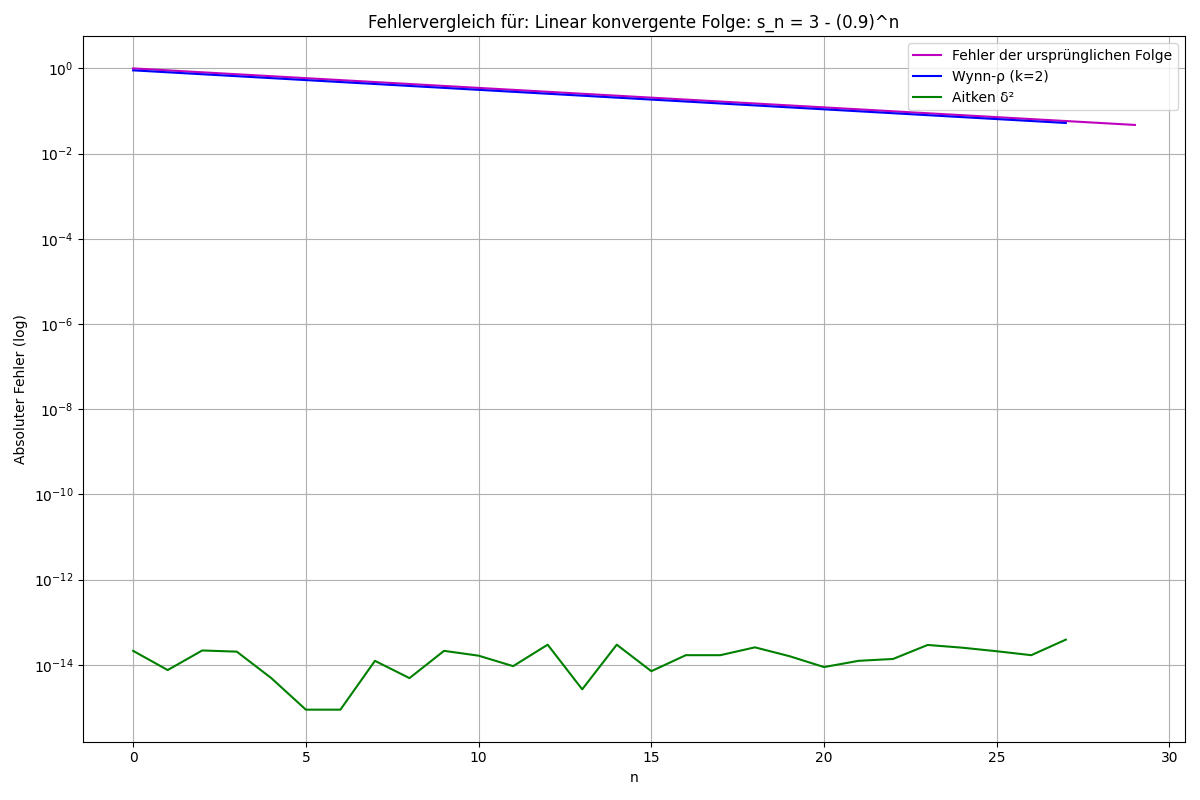
\includegraphics[width=\textwidth]{aitkenvsrho.png}\\
Während der Fehler beim Aitken-$\Delta^2$-Verfahren sehr schnell sehr klein ist, verhält sich der Fehler der $\rho$-Folge genau so wie der Fehler der originalen Folge $s_n$.

\newpage
\subsection{Alternierende Folgen: Vergleich von $\rho$ und $\epsilon$}\label{subsec:alternierend}
Die Stärken und Schwächen des $\epsilon$-Algorithmus werden in [\cite[112-115]{wynn1966convergence}] genauer erläutert. Der $\epsilon$-Algorithmus ist besonders effizient bei der Beschleunigung von alternierenden Folgen. Der $\rho$-Algorithmus führt hierbei zu kaum einer Verbesserung. Wir betrachten dafür die Leibniz-Reihe und vergleichen den $\epsilon$-Algorithmus mit dem $\rho$-Algorithmus:
\[
\sum_{k=0}^{\infty} (-1)^k \frac{1}{2k + 1} = \frac{\pi}{4}
\]
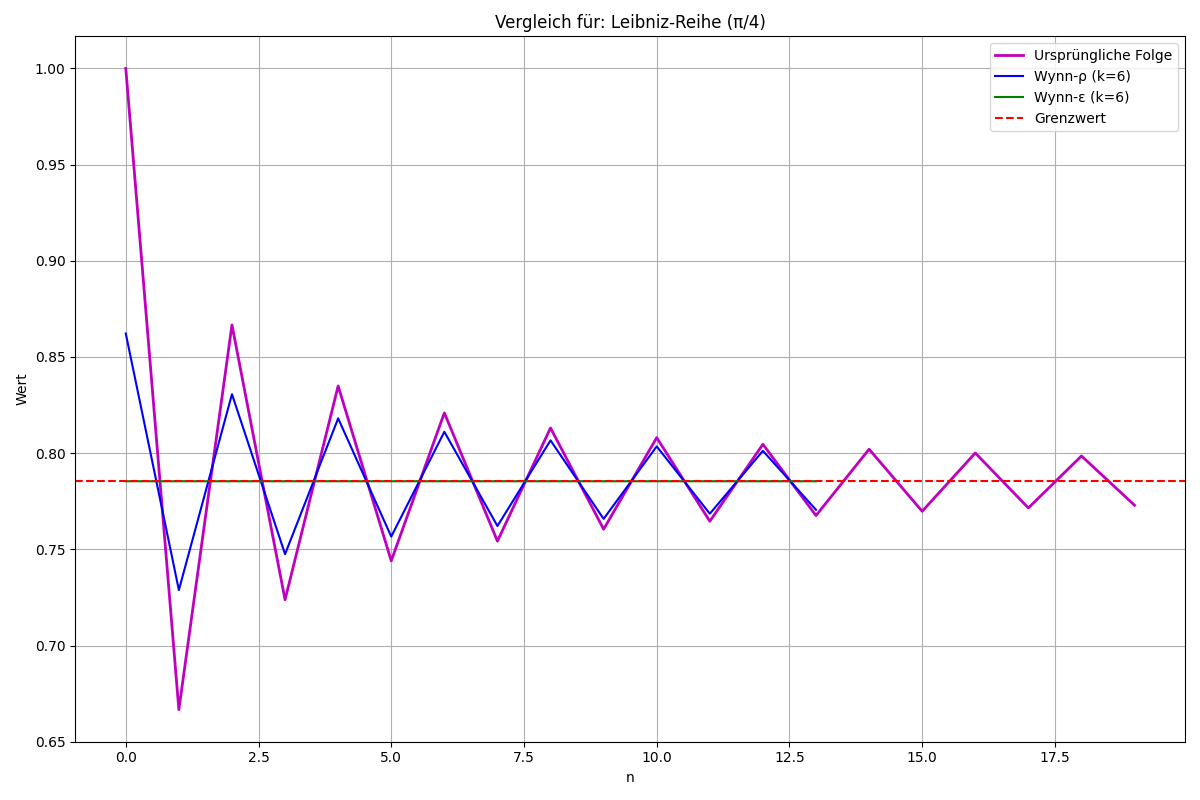
\includegraphics[width=\textwidth]{epsilonvsrho.png}
\\
Der $\epsilon$-Algorithmus erzielt schon in $n=0$ einen sehr genauen Wert, während der $\rho$-Algorithmus sich an die Originalfolge annähert.

\newpage
\subsection{Logarithmisch konvergente Folgen}\label{subsec:log}
Der $\rho$-Algorithmus zeigt seine besondere Stärke bei der Beschleunigung logarithmisch konvergenter Folgen. Wir betrachten dabei die sogenannte $Euler-Mascheroni-Konstante$ welche beschrieben wird durch
\[
\lim_{n \to \infty}\sum\limits_{k=1}^{n}\frac{1}{k}-ln(n) \approx0,57721566
\]
Wir verwenden hier keine Grafik, da wir ausschließlich die Genauigkeit des $\rho$-Algorithmus analysieren wollen. Für den Algorithmus ergeben sich dann folgende Werte:\\\\
\begin{tabular}{c|r|r|r|r|r}
$n$ & $k=-1$ & $k=0$ & $k=2$ & $k=4$ & $k=6$ \\
\hline
0 & 0.00000000 & 1.00000000 & 0.\underline{57}660033 & 0.\underline{5772}8341 & 0.\underline{577215}75 \\
1 & 0.00000000 & 0.80685282 & 0.\underline{57}692144 & 0.\underline{5772}2282 & 0.\underline{5772156}7 \\
2 & 0.00000000 & 0.73472104 & 0.\underline{577}06845 & 0.\underline{5772}1759 & 0.\underline{57721566} \\
3 & 0.00000000 & 0.69703897 & 0.\underline{577}13320 & 0.\underline{5772}1638 & 0.\underline{57721566} \\
4 & 0.00000000 & 0.67389542 & 0.\underline{577}16520 & 0.\underline{577215}98 & 0.\underline{57721566} \\
5 & 0.00000000 & 0.65824053 & 0.\underline{577}18265 & 0.\underline{577215}82 & 0.\underline{57721566} \\
6 & 0.00000000 & 0.64694699 & 0.\underline{577}19292 & 0.\underline{577215}75 & 0.\underline{57721566} \\
7 & 0.00000000 & 0.63841560 & 0.\underline{577}19935 & 0.\underline{577215}72 & 0.\underline{57721566} \\
8 & 0.00000000 & 0.63174368 & 0.\underline{5772}0357 & 0.\underline{577215}70 & 0.\underline{57721566} \\
9 & 0.00000000 & 0.62638316 & 0.\underline{5772}0646 & 0.\underline{577215}69 & 0.\underline{57721566} \\
10 & 0.00000000 & 0.62198207 & 0.\underline{5772}0850 & 0.\underline{577215}68 & 0.\underline{57721566} \\

\end{tabular}\\\\\\
Wir erreichen dementsprechend das exakte Ergebnis bereits in Rekursionsschritt $k=6$ mit Tiefe $n=2$.




\newpage
\subsection{Langsam konvergente Folgen}\label{subsec:langsam}
Ebenso spannend gestaltet sich das Verhalten des $\rho$-Algorithmus bei Anwendung auf die Zeta-Funktion:
% Um das zu veranschaulichen, vergleichen wir ihn mit dem $\epsilon$-Algorithmus, welcher hier große Schwierigkeiten hat. Dafür betrachten wir die $\zeta-$Funktion in Reihendarstellung:
\[
\zeta(s) = \sum_{n=1}^{\infty} \frac{1}{n^s}
\]
Diese konvergiert besonders langsam, wenn $s\downarrow1$. Dafür vergleichen wir den $\rho$-Algorithmus mit dem $\epsilon$-Algorithmus, welcher hier große Schwierigkeiten hat. In der Grafik sei $s=1,5$ der Beispielwert.\\\\
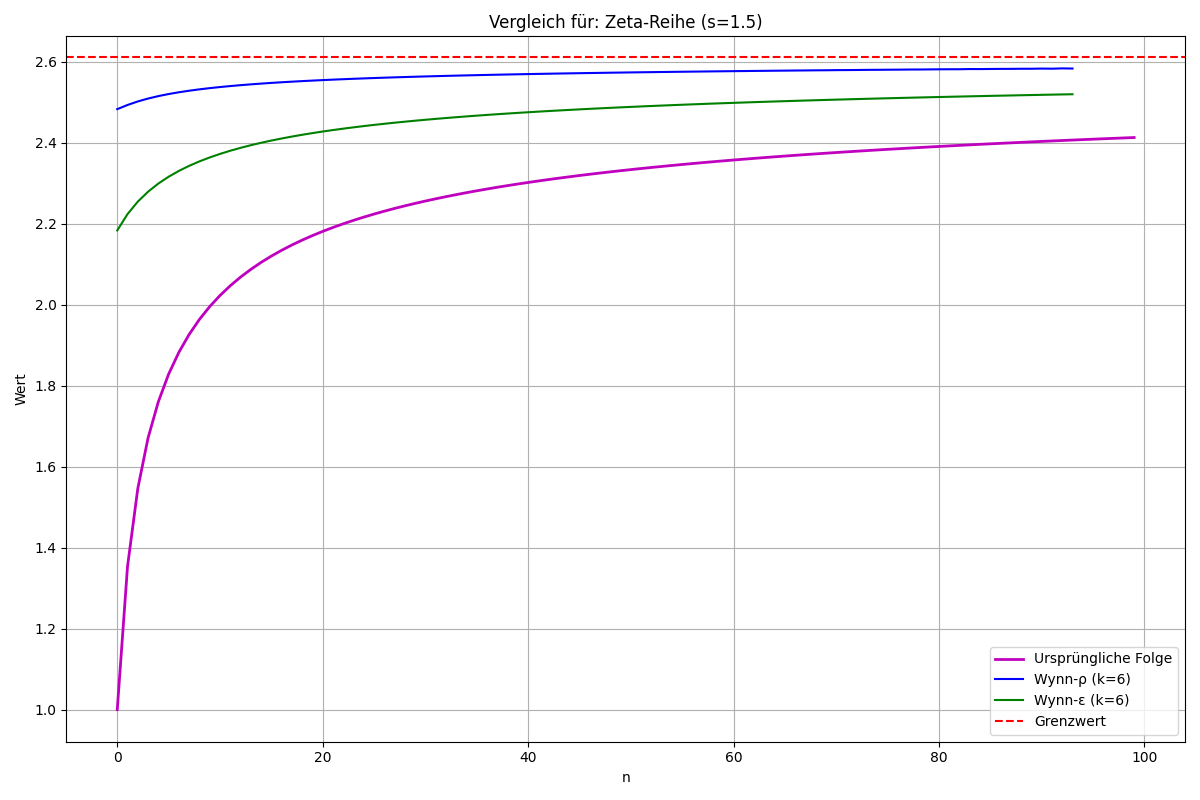
\includegraphics[width=\textwidth]{zetaepsvsrho.png}
\\
Es wird hier gut erkennbar, dass der $\rho$-Algorithmus im Vergleich noch sehr gut abschneidet, doch auch hier die Beschleunigung schon etwas schwerer gelingt. Bei noch stärkerer Annäherung an $s=1$ nimmt die Effizienz des Algorithmus weiter ab. Diesem Problem wollen wir in \secref{subsubsec:mod1} entgegenwirken.

\newpage
\subsection{Modifikationen}\label{subsec:modifikationen}
Für die folgenden beiden Modifikationen beziehen wir uns auf [\cite[376-378]{sidi2003practical}], im folgenden Text finden sich jeweils nur die Definitionen mit einem Anwendungsbeispiel.\\
Durch eine kleine Veränderung der ursprünglichen Definition können wir in einigen Fällen sehr starke Verbesserungen erzielen. Im Wesentlichen verändern wir hier den Term, der in der klassischen Definition die Interpolationspunkte beschreibt \eqref{eq:rhodef}, welche standardmäßig mit $(k+1)$ definiert werden.
\subsubsection{Modifikation 1 - $\rho(\gamma)$-Algorithmus}\label{subsubsec:mod1}
\textbf{Definition:}
\begin{align*}
\overline\rho^{(n)}_{-1} &= 0 \quad\\
\overline\rho^{(n)}_0 &= s_n \\
\overline\rho^{(n)}_{k+1} &= \overline\rho^{(n+1)}_{k-1} + \frac{k - \gamma}{\overline\rho^{(n+1)}_{k} - \overline\rho^{(n)}_k}
\end{align*}
% \textbf{Konvergenzgeschwindigkeit:}\\
% \textit{
% Sei $\gamma \notin \mathbb{N}$. Dann gilt:\\
% \begin{align*}
% \overline\rho^{(n)}_{2k}-s\approx\sum\limits_{i=0}^\infty w_{ki}j^{\gamma-2k-i}, \quad n\rightarrow\infty
% \end{align*}}
\subsubsection*{Leibniz-Reihe}
Wenn wir diesen Algorithmus nun mit bestimmtem $\gamma$ auf die $Leibniz$-$Reihe$ anwenden, erzielen wir im Gegensatz zum klassischen Algorithmus eine starke Verbesserung der Konvergenz. Dazu betrachten wir das Beispiel der Alternierenden Harmonischen Reihe:\\
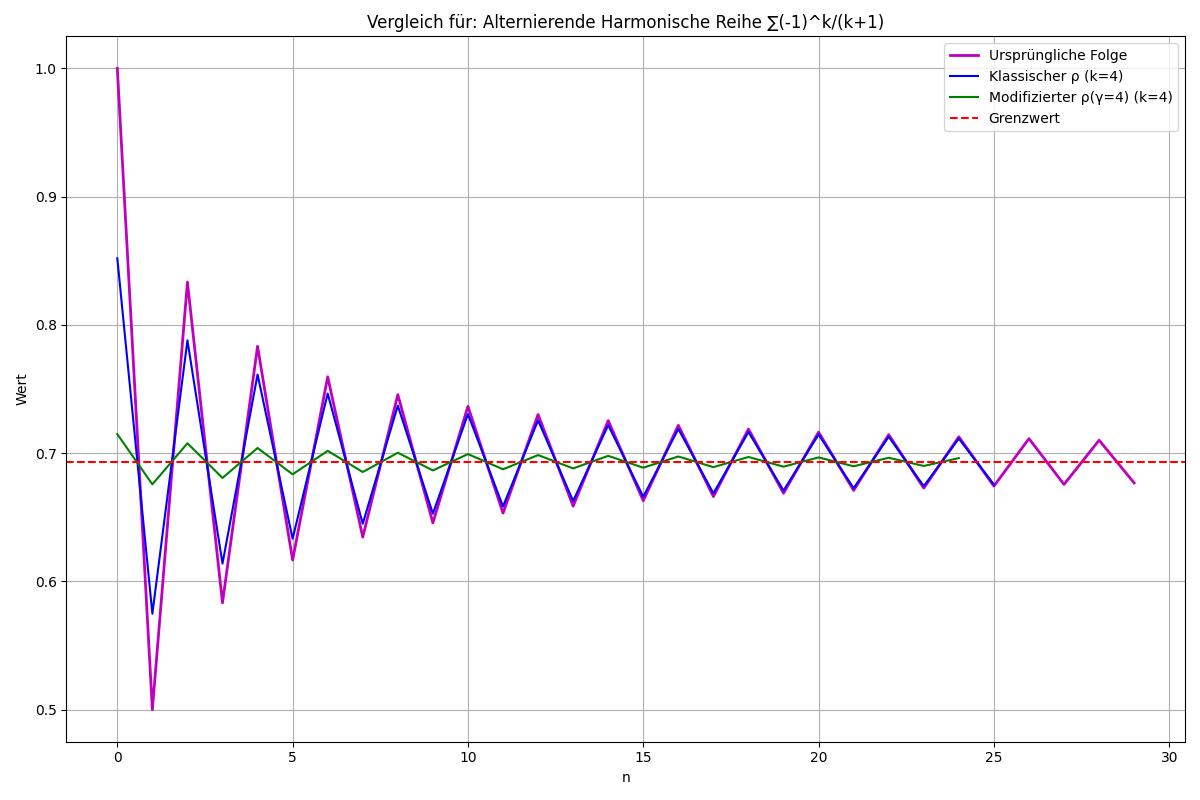
\includegraphics[width=\textwidth]{modi1.png}
Wir erkennen hier eine sehr starke Verbesserung im Vergleich zum ursprünglichen Algorithmus. Wählen wir nun unser $\gamma$ noch größer, nähern wir uns immer stärker dem tatsächlichen Grenzwert an.
\subsubsection*{Zeta-Funktion}
In \secref{subsec:langsam} haben wir eine eingeschränkte Beschleunigung für die Zeta-Funktion durch den $\rho$-Algorithmus bereits festgestellt. Durch geeignete Wahl der Parameter können wir das jedoch optimieren.\\\\
Der exakte Wert ist 
\[
\zeta(1,1)=10,58444846
\]
Während der klassische $\rho$-Algorithmus bei einer Rekursionstiefe von $n=23$ noch einen Fehler von $(e_{23}>5)$ aufweist, kann unser modifizierter $\rho(\gamma)$-Algorithmus mit dem Parameter $\gamma=0,9$ einen Fehler von $(e_{23}^{\gamma}\approx10^{-8})$ erzielen.

Hierbei ist der Parameter sehr sorgfältig zu wählen; kleine Abweichungen können in diesem Fall die Beschleunigung völlig ruinieren.\\
\begin{center}
\begin{tabular}{c|c|c|c}
$n$ & Original & $\rho$ (standard)& $\rho(\gamma=0,9)$ \\ \hline
0 & 1.00000000 & 4.05905983 & \underline{10.584}39421 \\ 
1 & 1.46651650 & 4.21881639 & \underline{10.5844}2870 \\ 
2 & 1.76516932 & 4.34421820 & \underline{10.5844}3969 \\ 
3 & 1.98280696 & 4.44700181 & \underline{10.58444}402 \\ 
4 & 2.15307494 & 4.53383717 & \underline{10.58444}598 \\ 
5 & 2.29240141 & 4.60885546 & \underline{10.58444}697 \\ 
6 & 2.40999730 & 4.67478432 & \underline{10.58444}752 \\ 
7 & 2.51152885 & 4.73351524 & \underline{10.58444}784 \\ 
8 & 2.60072236 & 4.78641165 & \underline{10.584448}03 \\ 
9 & 2.68015518 & 4.83448760 & \underline{10.584448}16 \\ 
10 & 2.75168186 & 4.87851702 & \underline{10.584448}24 \\ 
11 & 2.81667995 & 4.91910356 & \underline{10.584448}30\\ 
12 & 2.87619987 & 4.95672683 & \underline{10.584448}34 \\ 
13 & 2.93106029 & 4.99177397 & \underline{10.584448}37 \\ 
14 & 2.98191131 & 5.02456188 & \underline{10.584448}39 \\ 
... & ... & ... & ... \\
23 & 3.32204995 & 5.25044529 & \underline{10.5844484}5
\end{tabular}
\end{center}
\subsubsection{Automatisierter $\rho(\gamma)$-Algorithmus}
Folgend soll noch ein kurzer Einblick in eine mögliche Automatisierung des $\rho(\gamma)$-Verfahrens gegeben werden. Weitere Ausführungen zur Automatisierung und zur Verbindung zu anderen Beschleunigungsverfahren lassen sich in [\cite[378]{sidi2003practical}] nachlesen.

Der automatisierte $\rho(\gamma)$-Algorithmus beschleunigt die Konvergenz von Folgen $\{s_n\}$ durch adaptive Parameterschätzung.\\\\
Die Idee ist, dass für Folgen mit asymptotischem Verhalten
\[ s_n \sim s + \sum_{i=0}^\infty \alpha_i n^{\gamma-i} \quad (n\to\infty) \]
der Algorithmus automatisch den optimalen Parameter $\gamma'$ bestimmt und den $\rho(\gamma')$-Algorithmus anwendet.

\subsubsection*{Algorithmus}
\begin{enumerate}
\item {Parameterschätzung}:
\begin{itemize}
\item Eingabe: $s_0,\ldots,s_r$
\item Wende $\rho(-2)$-Algorithmus auf Hilfsfolge $\{\gamma_m\}_{m=0}^{r-2}$ an
\item Setze:
  \[ \gamma' = \begin{cases}
  \bar{\rho}_{2k}^{(0)} & \text{für } r=2k+2 \\
  \bar{\rho}_{2k}^{(1)} & \text{für } r=2k+3
  \end{cases} \]
\end{itemize}

\item {Konvergenzbeschleunigung}:
\begin{itemize}
\item Wende $\rho(\gamma')$-Algorithmus auf $\{s_n\}$ an
\item Ausgabe: Beschleunigte Näherungen $\bar{\rho}_{2k}^{(j)}$ für $0\leq j+2k\leq r$
\end{itemize}
\end{enumerate}
Der große Vorteil liegt hier darin, dass keine Schätzung des $\gamma$-Parameters nötig ist.


\subsubsection{Modifikation 2 - $\rho(\gamma,p)$-Algorithmus}\label{subsubsec:mod2}
\textbf{Definition:}
\begin{align*}
\hat\rho^{(n)}_{-1} &= 0 \quad\\
\hat\rho^{(n)}_0 &= s_n \\
\hat\rho^{(n)}_{k+1} &= \hat\rho^{(n+1)}_{k-1} + \frac{C_k^{(\gamma,p)}}{\hat\rho^{(n+1)}_{k} - \hat\rho^{(n)}_k}
\end{align*}

wobei
\begin{align*}
C_{2k}^{(\gamma,p)}&=-\gamma+\frac{k}{p},\quad C_{2k+1}^{(\gamma,p)}=-\gamma+\frac{k}{p}+1
\end{align*}
Die Abweichung zu Modifikation 1 bezieht sich auf den Zähler der 3. Gleichung. Der Schritt $k$ wird skaliert um $\frac{1}{p}$. Das führt unter Umständen zu einer weiteren kleinen Verbesserung im Vergleich zu Modifikation 1. Dazu betrachten wir das Beispiel der Alternierenden Harmonischen Reihe:\\
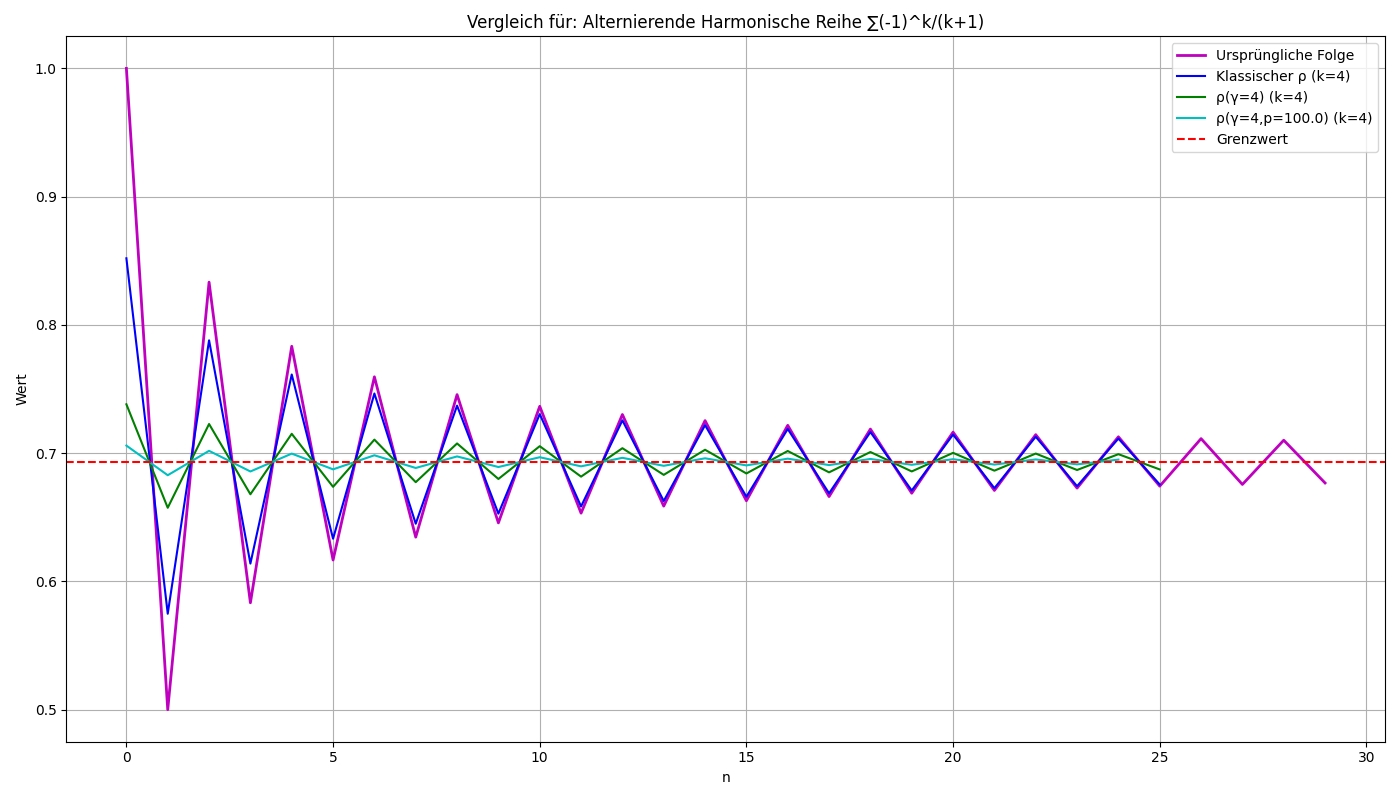
\includegraphics[width=\textwidth]{modi2.png}
Es zeigt sich in den Anwendungen, dass sich eine grobe Verbesserung durch das Verändern des $\gamma$-Parameters erzielen lässt, der Parameter $p$ bezweckt hier nur eine minimale Verbesserung um $\approx 10^{-6}$.

\newpage
\printbibliography[heading=bibintoc, title={Literaturverzeichnis}]

\end{document}